\documentclass{sigchi}

% Use this section to set the ACM copyright statement (e.g. for
% preprints).  Consult the conference website for the camera-ready
% copyright statement.

% Copyright
%\CopyrightYear{2016}
%%\setcopyright{acmcopyright}
%\setcopyright{acmlicensed}
%%\setcopyright{rightsretained}
%%\setcopyright{usgov}
%%\setcopyright{usgovmixed}
%%\setcopyright{cagov}
%%\setcopyright{cagovmixed}
%% DOI
%\doi{http://dx.doi.org/10.475/123_4}
%% ISBN
%\isbn{123-4567-24-567/08/06}
%%Conference
%\conferenceinfo{CHI'16,}{May 07--12, 2016, San Jose, CA, USA}
%%Price
%\acmPrice{\$15.00}

% Use this command to override the default ACM copyright statement
% (e.g. for preprints).  Consult the conference website for the
% camera-ready copyright statement.

%% HOW TO OVERRIDE THE DEFAULT COPYRIGHT STRIP --
%% Please note you need to make sure the copy for your specific
%% license is used here!
% \toappear{
% Permission to make digital or hard copies of all or part of this work
% for personal or classroom use is granted without fee provided that
% copies are not made or distributed for profit or commercial advantage
% and that copies bear this notice and the full citation on the first
% page. Copyrights for components of this work owned by others than ACM
% must be honored. Abstracting with credit is permitted. To copy
% otherwise, or republish, to post on servers or to redistribute to
% lists, requires prior specific permission and/or a fee. Request
% permissions from \href{mailto:Permissions@acm.org}{Permissions@acm.org}. \\
% \emph{CHI '16},  May 07--12, 2016, San Jose, CA, USA \\
% ACM xxx-x-xxxx-xxxx-x/xx/xx\ldots \$15.00 \\
% DOI: \url{http://dx.doi.org/xx.xxxx/xxxxxxx.xxxxxxx}
% }

% Arabic page numbers for submission.  Remove this line to eliminate
% page numbers for the camera ready copy
% \pagenumbering{arabic}

% Load basic packages
\usepackage{balance}       % to better equalize the last page
\usepackage{graphics}      % for EPS, load graphicx instead 
\usepackage[T1]{fontenc}   % for umlauts and other diaeresis
\usepackage{txfonts}
\usepackage{mathptmx}
\usepackage[pdflang={en-US},pdftex]{hyperref}
\usepackage{color}
\usepackage{booktabs}
\usepackage{textcomp}

\usepackage{hyperref}
\usepackage{url}
\usepackage{float}
\usepackage{graphicx, subcaption}

% Some optional stuff you might like/need.
\usepackage{microtype}        % Improved Tracking and Kerning
% \usepackage[all]{hypcap}    % Fixes bug in hyperref caption linking
\usepackage{ccicons}          % Cite your images correctly!
% \usepackage[utf8]{inputenc} % for a UTF8 editor only

% If you want to use todo notes, marginpars etc. during creation of
% your draft document, you have to enable the "chi_draft" option for
% the document class. To do this, change the very first line to:
% "\documentclass[chi_draft]{sigchi}". You can then place todo notes
% by using the "\todo{...}"  command. Make sure to disable the draft
% option again before submitting your final document.
\usepackage{todonotes}

% Paper metadata (use plain text, for PDF inclusion and later
% re-using, if desired).  Use \emtpyauthor when submitting for review
% so you remain anonymous.
\def\plaintitle{Context-aware Communication in the Car}
\def\plainauthor{First Author, Second Author, Third Author,
  Fourth Author, Fifth Author, Sixth Author}
\def\emptyauthor{}
\def\plainkeywords{Authors' choice; of terms; separated; by
  semicolons; include commas, within terms only; required.}
\def\plaingeneralterms{Documentation, Standardization}

% llt: Define a global style for URLs, rather that the default one
\makeatletter
\def\url@leostyle{%
  \@ifundefined{selectfont}{
    \def\UrlFont{\sf}
  }{
    \def\UrlFont{\small\bf\ttfamily}
  }}
\makeatother
\urlstyle{leo}

% To make various LaTeX processors do the right thing with page size.
\def\pprw{8.5in}
\def\pprh{11in}
\special{papersize=\pprw,\pprh}
\setlength{\paperwidth}{\pprw}
\setlength{\paperheight}{\pprh}
\setlength{\pdfpagewidth}{\pprw}
\setlength{\pdfpageheight}{\pprh}

% Make sure hyperref comes last of your loaded packages, to give it a
% fighting chance of not being over-written, since its job is to
% redefine many LaTeX commands.
\definecolor{linkColor}{RGB}{6,125,233}
\hypersetup{%
  pdftitle={\plaintitle},
% Use \plainauthor for final version.
%  pdfauthor={\plainauthor},
  pdfauthor={\emptyauthor},
  pdfkeywords={\plainkeywords},
  pdfdisplaydoctitle=true, % For Accessibility
  bookmarksnumbered,
  pdfstartview={FitH},
  colorlinks,
  citecolor=black,
  filecolor=black,
  linkcolor=black,
  urlcolor=linkColor,
  breaklinks=true,
  hypertexnames=false
}

% create a shortcut to typeset table headings
% \newcommand\tabhead[1]{\small\textbf{#1}}

% End of preamble. Here it comes the document.
\begin{document}

\title{\plaintitle}

\numberofauthors{3}
\author{%
  \alignauthor{Tobias Martin\\
    \affaddr{University of Munich (LMU)}\\
    \affaddr{Munich, Germany}\\
    \email{t.martin@campus.lmu.de}}\\
  \alignauthor{Stefan Lang\\
    \affaddr{University of Munich (LMU)}\\
    \affaddr{Munich, Germany}\\
    \email{stefan.lang@campus.lmu.de}}\\
  \alignauthor{Simon Weiser\\
    \affaddr{University of Munich (LMU)}\\
    \affaddr{Munich, Germany}\\
    \email{simon.weiser@campus.lmu.de}}\\
}

\maketitle

\begin{abstract}
TODO: put text here
\end{abstract}

\category{H.5.2}{Information Interfaces and Presentation (e.g., HCI)}{User Interfaces --- \textit{Prototyping}}
\category{H.4.3}{Information Systems Applications}{Communications Applications}

\keywords{Automotive user interfaces, calling while driving, context sharing, driving safety, phone call.}

\section{Introduction}
TODO: put text here

\section{Related Work}
TODO: put text here

\section{Concept}
TODO: put text here

\section{Implementation}

We designed a simple and ordinary contacts app which is enhanced by displaying the context of the person you want to call. For our goal the term context means to consider mostly all of these information:
\newline

\begin{center}
\begin{table}[htbp]
\begin{center}
\begin{tabular}[center]{l}
\toprule
Context Information\\
\midrule
Activity \\
Road Type \\
Destination \\
Remaining Travel Time \\
Position \\
Hands-free Speaking \\
Speed \\
Weather \\
\bottomrule
\end{tabular}
\end{center}
\caption[Context Information]{Context Information.\label{tab:cont}}
\end{table}
\end{center}

First of all you want to know what the person you want to call is doing at the moment. We distinguished between the activities \textit{driving}, \textit{cycling} and \textit{still} where the latter means the person to call is doing nothing right now and his/her device is motionless on a table for example. Depending on if someone is driving you want to have the listed additional information. One would be the road type which lets you know if someone is driving e.g. in a city or on a highway etc. Another one is the destination the person is heading to and the remaining travel time. Therefore you need the person's position. This could either be a pinpoint GPS-coordinate, or if the user does not want to share his exact location, just a radius or a place name of his current position. Another very important aspect of the person's context is if hands-free speaking is enabled or disabled while in the car. 

Besides information about the speed and the current weather situation are helpful to know. At the current state of our app all of these information can be accessed automatically except the destination and the remaining travel time, which have to be typed in manually.

\subsection{App Design}
The Android-App we build basically consists of two different views, an overview and a detail view (see figure \ref{fig:app}).
\newline
\begin{figure}[H]
\centering
\begin{subfigure}{.23\textwidth}
  \centering
  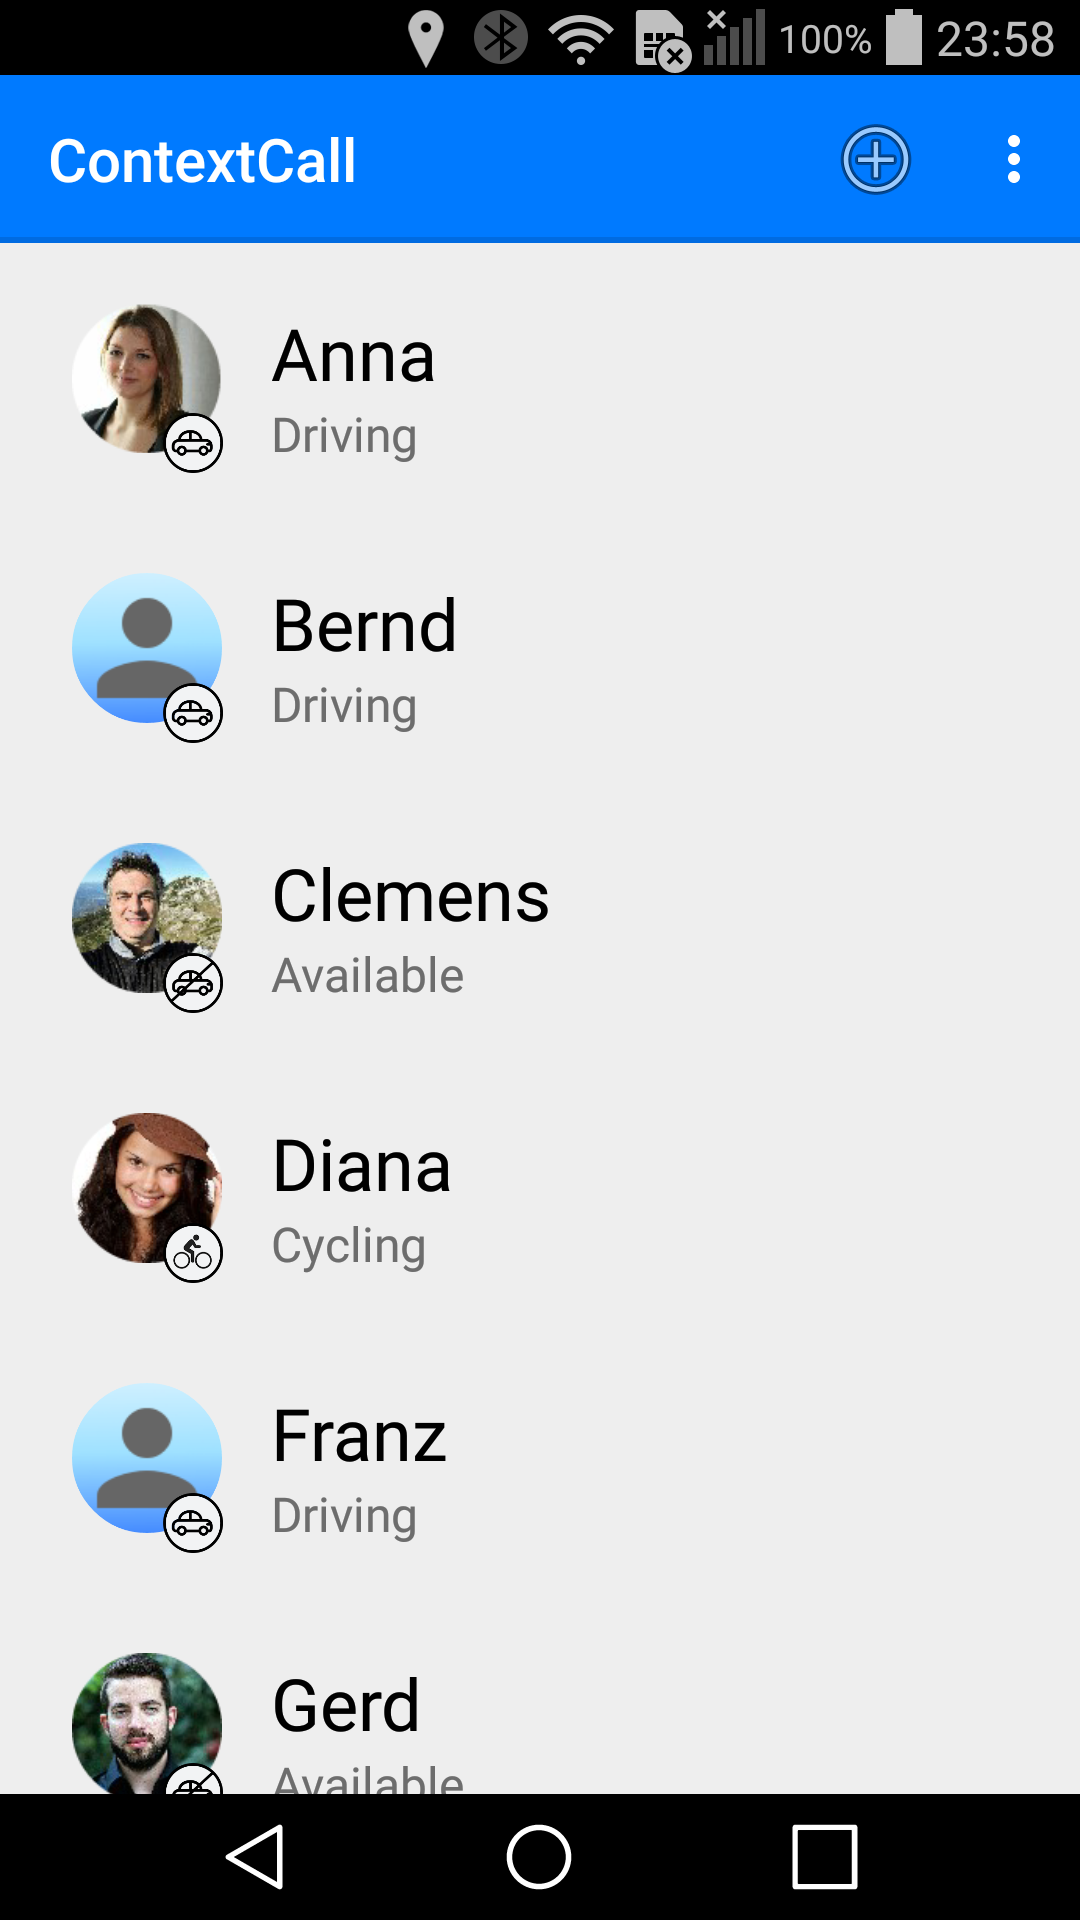
\includegraphics[width=.7\linewidth]{figures/app_1}
  \caption{Overview}
  \label{fig:app_1}
\end{subfigure}
\begin{subfigure}{.23\textwidth}
  \centering
  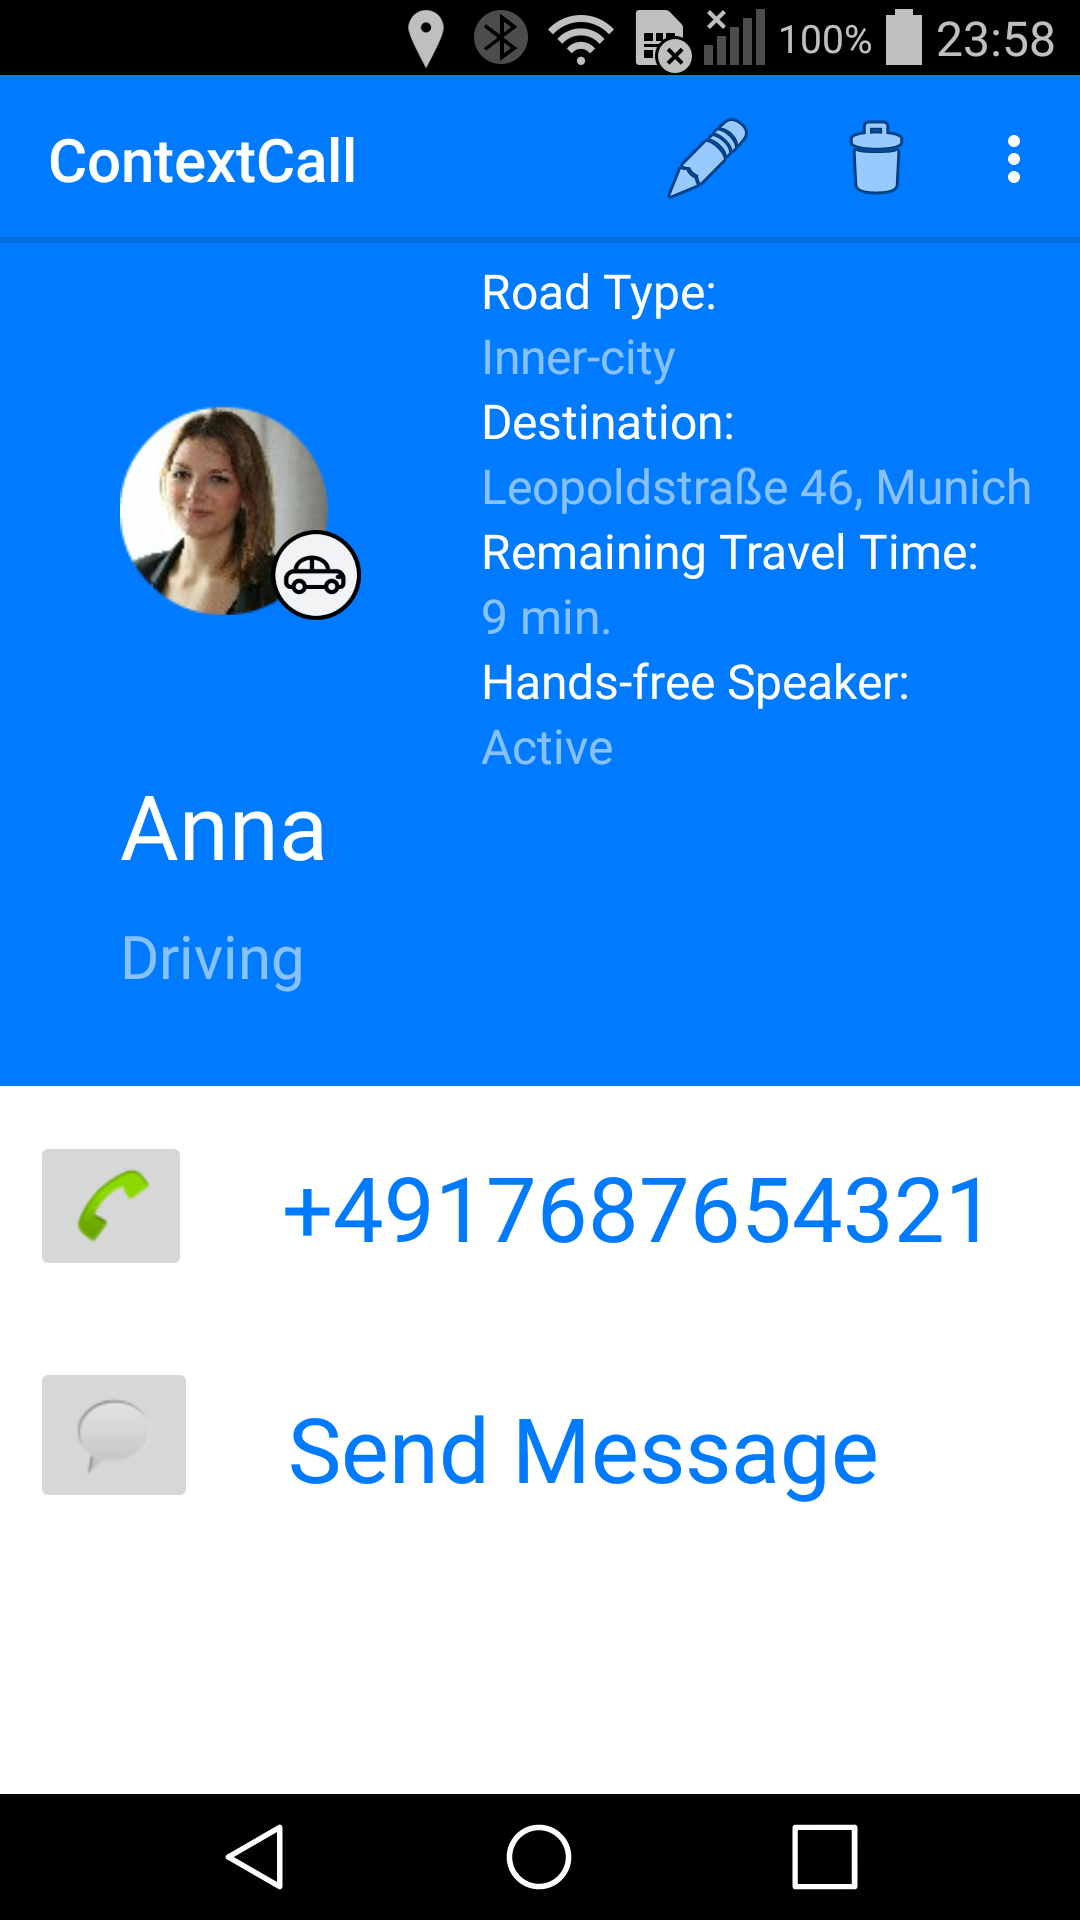
\includegraphics[width=.7\linewidth]{figures/app_2}
  \caption{Detailview}
  \label{fig:app_2}
\end{subfigure}
\caption{Android Application ContextCall}
\label{fig:app}
\end{figure}

On the overview on the left you see all your contacts as you know it from other contacts apps, but with the additional information about a person's activity, which is shown by the icons next to the image and the string below the name. By taping on a contact, the detail view appears and shows the additional context information mentioned in table \ref{tab:cont}. The particular case in figure \ref{fig:app_2} for example gives information about the road type, the destination and the remaining travel time. Furthermore you get informed that hands-free speaking is enabled. If you then decide to call 'Anna' although she is driving, a small alert pops up and gives you three options (see figure \ref{fig:app_3}). You can either call her or not, or you make use of the '\textit{remind me}'-option which notifies you when her status is 'still'.
\begin{figure}[H]
  \centering
  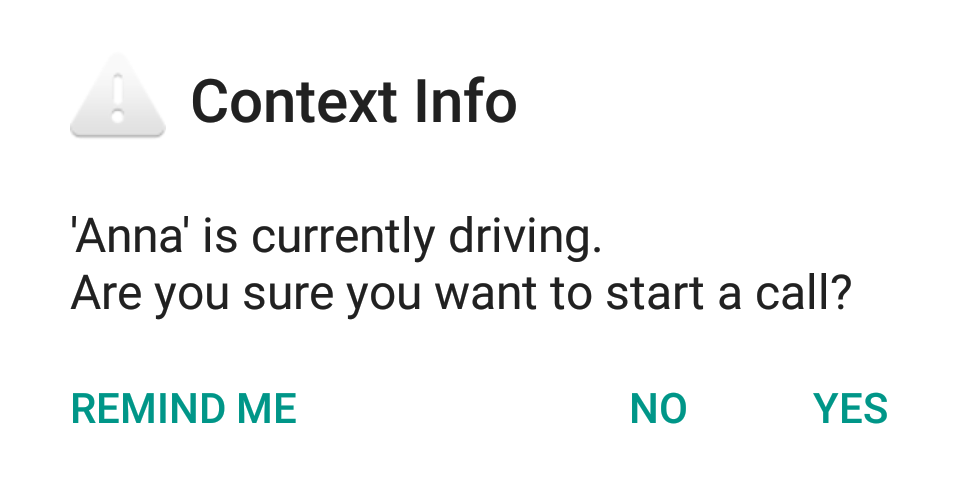
\includegraphics[width=.55\columnwidth]{figures/app_3}
  \caption{Alert Pop-Up}~\label{fig:app_3}
\end{figure}
At the beginning we implemented most of the context recognition by our own. We used for example GPS to find out if someone is driving. If someone's speed was over 10 kilometers per hour we set the status to 'driving'. But in mid-May of 2016 Google released its new so-called \textit{Awareness API}\footnote{https://developers.google.com/awareness/} which made things much easier for us as programmers. From this point on we were able to get the activity of a user by only a few lines of code and this API became the core of our application.

The Awareness API is part of the \textit{Google Play Services} and is a unified sensing platform, enabling apps to be aware of all aspects of a user's context, while managing system health for you \cite{you16}. With this API your app is able to recognize the following 7 different context types \cite{goo16}:
\begin{description}
\item[Location]
The user's current location as a latitude and longitude value.
\item[Place]
A semantic version of a location that is called place (including the place type, e.g. a coffee shop).
\item[Beacons]
What is around a user? Are there nearby beacons that can be detected and identified?
\item[Time]
The local time of a user that can be combined with other context information to form a more complex condition.
\item[Headphones' State]
Are headphones plugged in the device or not?
\item[Weather]
Ambient conditions like the weather, which have an effect on the user's behavior.
\item[Activity]
The detected user activity (e.g. walking, running, biking and driving)
\end{description}

The latter of these is the important one for the goal of activity and context recognition. All of these information can be combined using \textit{AND}, \textit{OR}, and \textit{NOT} boolean operators to build complicated conditions that have to be met to trigger a notification. E.g. you can construct a condition that says that the user is driving in the car AND he is near a pharmacy AND it is during the opening hours of that shop. If these requirements are fulfilled, then you tell the user that he can pick up the wanted medication.

In particular, we used the \textit{Fence API}\footnote{https://developers.google.com/awareness/android-api/fence-api-overview}, which is part of the Awareness API. The concept of \textit{fences} is taken from Geo-Fencing, in which a geographic region, or "Geo- Fence", is defined, and an app receives callbacks when a user enters or leaves a region. Only that in this case it is not a region that is entered but an activity. So whenever the activity state transitions, it lets our app react to the user's current activity. For example, "Tell me whenever the user is driving". Once the conditions are met the app receives a callback and we can update the status of a user.





\section{User Study}
To evaluate our concept and the actual implementation we invited a total of 25 participants to our user study. As the overall goal was to evaluate if users perceive the context information provided by our application correctly, we decided to generate 10 different use-cases (scenarios). We vocally discussed each scenario with the current participant, but all the context information had to be pulled out from the running app on a provided smartphone. Differing by the call trigger (meaning the reason why a participant had to call a person) and the context the person being called (callee) is in, the participants had to decide whether they would like to: 

\begin{enumerate}
\item Make the call (or)
\item Not make the call (and)
\item Not make the call but send a text message (and/or)
\item Not make the call but get notified when the driver status changes
\end{enumerate}

Following the scenarios we asked additional questions with the participants acting the role of the driver (the person being called). Goal of these questions was to gather inside in the willingness of potential users to share more or less specific information.

The following figures visualise the outcome of our user study. Figure \ref{fig:WouldYouCall_1} to \ref{fig:WouldYouCall_3} focus on the 10 different scenarios which can be distinguished along the x-axis. As mentioned they differ in the status the callee is in (driving, cycling, still). Distribution of the answers given by our participants can be seen along the y-axis, while colours visualise the four possible choices.

\begin{figure}
\centering
  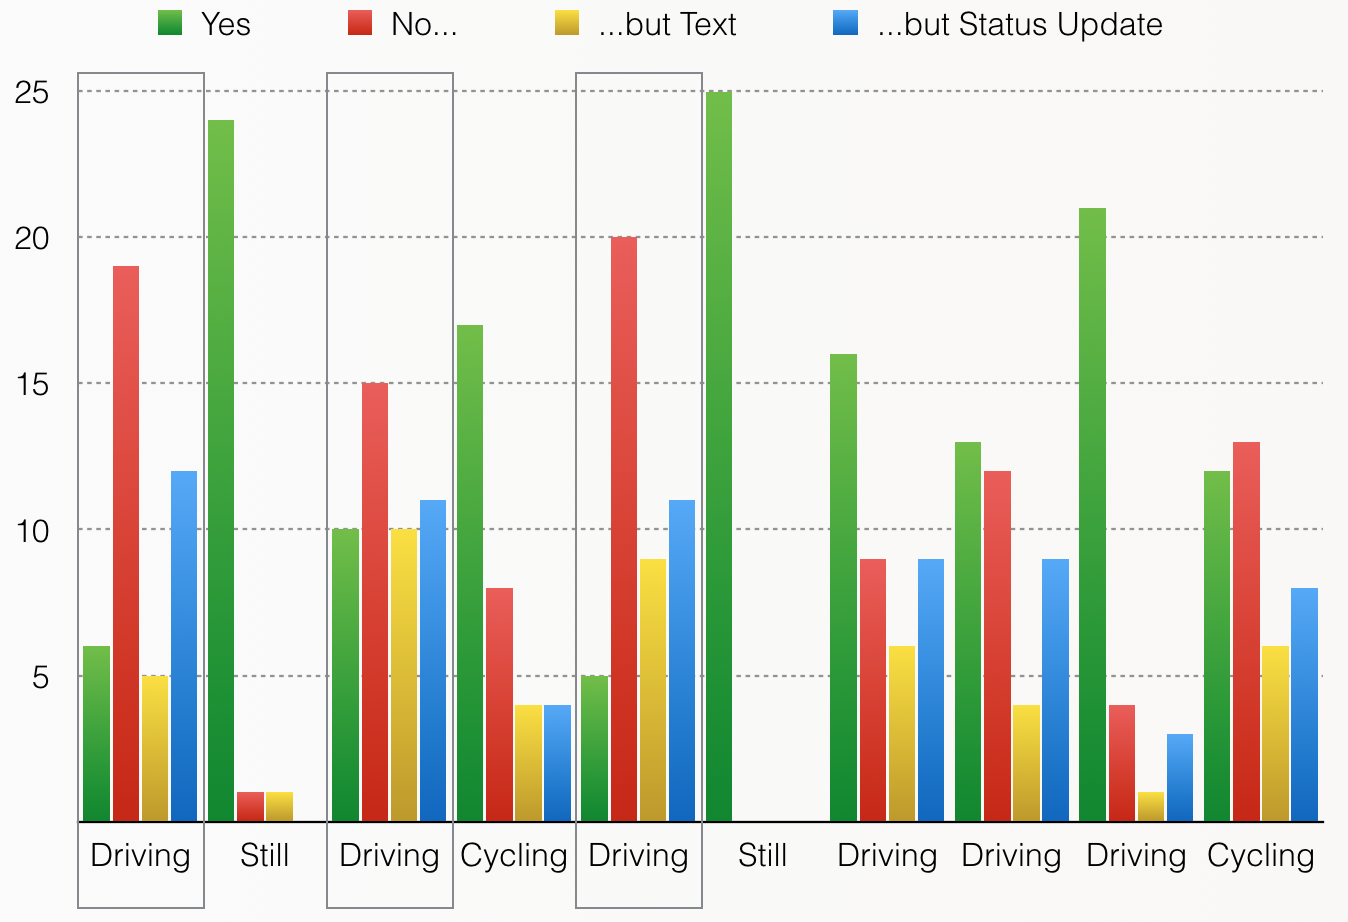
\includegraphics[width=0.9\columnwidth]{figures/WouldYouCall_1}
  \caption{User Study: Would you make the call (status driving)}~\label{fig:WouldYouCall_1}
\end{figure}

Highlighted in figure \ref{fig:WouldYouCall_1} you can see three different scenarios with the callee in the status 'driving'. As anticipated the majority of participants would not make a call in this situation (red bars). Moreover the majority would not like to send a text message straight away, or get notified if the status of the driver changes. Regarding our concept this outcome allows us to suppose that participants pulled the correct context information out of the app and that they consider the safety of the person they want to call.

\begin{figure}
\centering
  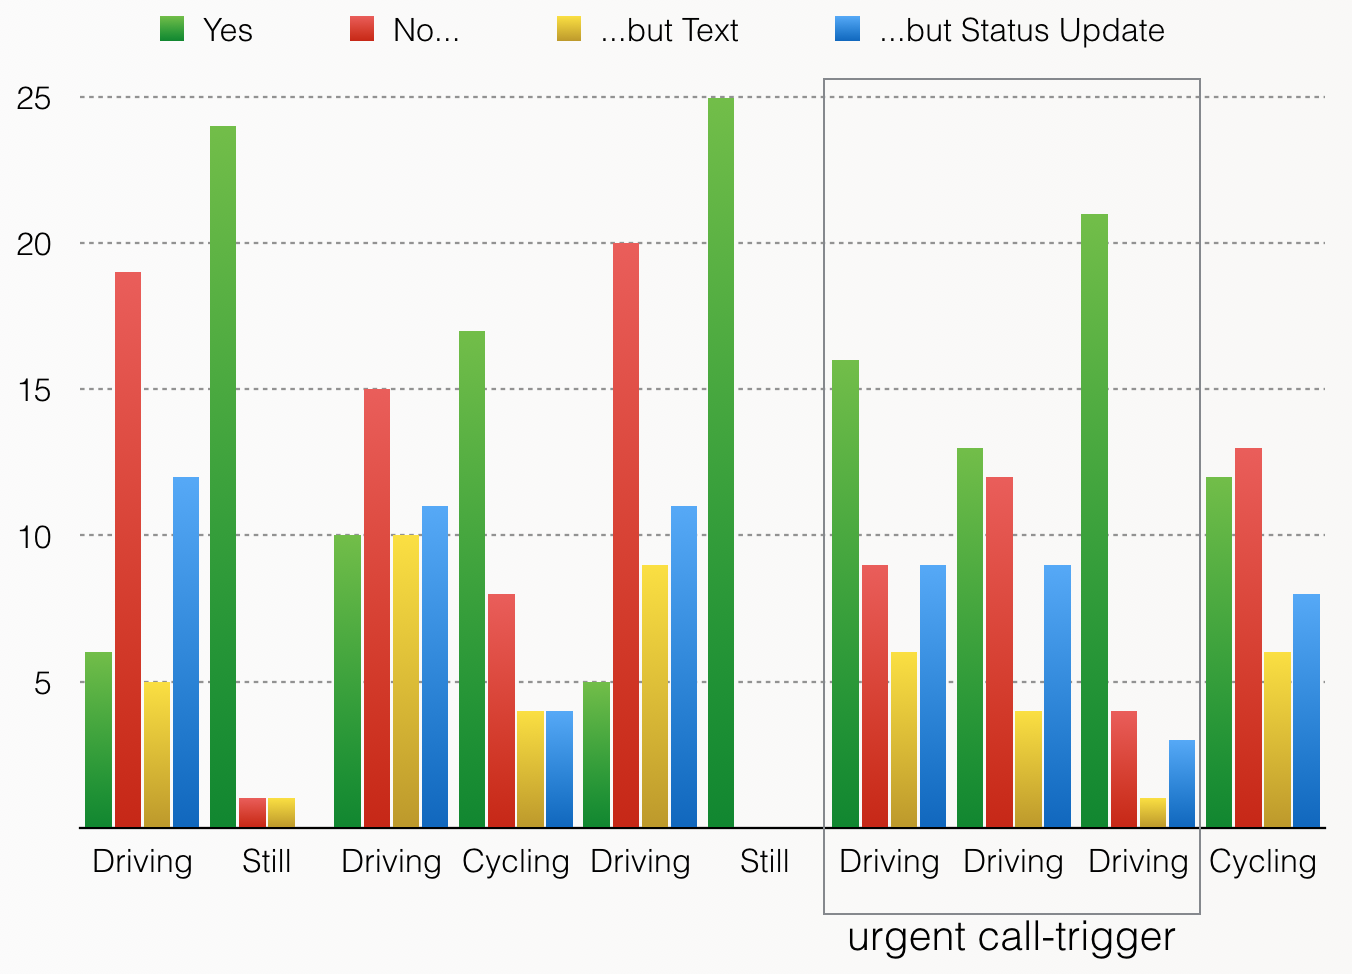
\includegraphics[width=0.9\columnwidth]{figures/WouldYouCall_2}
  \caption{User Study: Would you make the call (status driving/with urgent call-trigger)}~\label{fig:WouldYouCall_2}
\end{figure}

Contrary to the confirmed hypotheses shown in figure \ref{fig:WouldYouCall_1} (people will not make the call when they see the callee is driving), we found three 'driving' scenarios in which the participants would in fact make the call, although the callee is displayed as driving. Figure \ref{fig:WouldYouCall_2} focuses on these three scenarios with a majority of participants making the call (green bars). Discussion with our participants provided enough feedback to ensure that these decisions were based on the call-trigger (the reason they had to make the call). With call-triggers getting urgent (an emergency in the family for instance), people tend to ignore the context of the callee. Consulting with the participants we decided that users should always have the possibility to make calls in case of emergencies and that blocking calls completely is ineligible.

\begin{figure}
\centering
  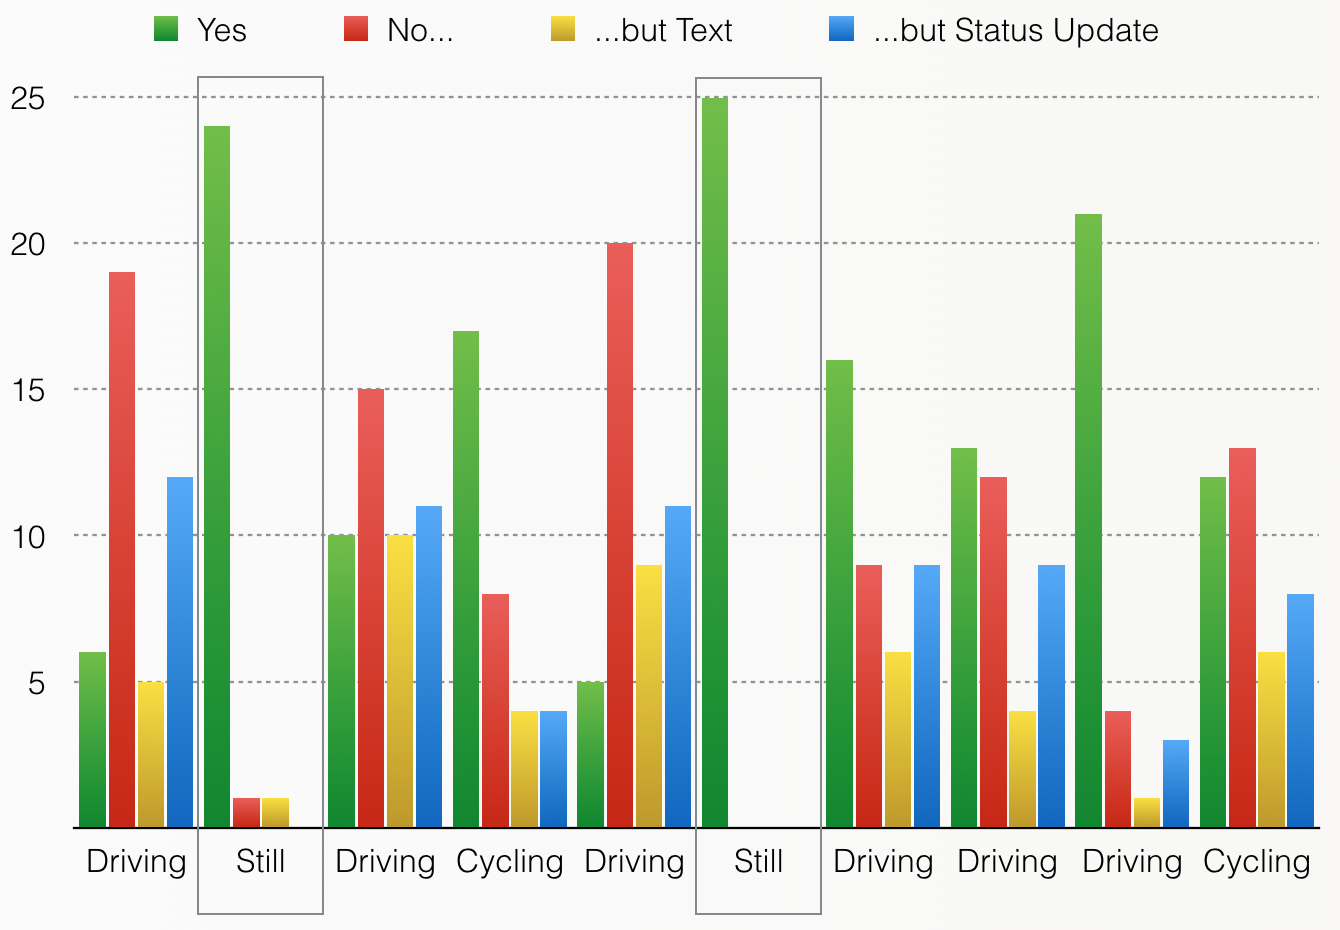
\includegraphics[width=0.9\columnwidth]{figures/WouldYouCall_3}
  \caption{User Study: Would you make the call (status still)}~\label{fig:WouldYouCall_3}
\end{figure}

To gain even more proof of our concept we generated two scenarios with the callee being in the status 'still'. Figure \ref{fig:WouldYouCall_3} focuses on these two scenarios and provides assurance that participants perceive our provided context information correctly and make their call straight away.

\begin{figure}
\centering
  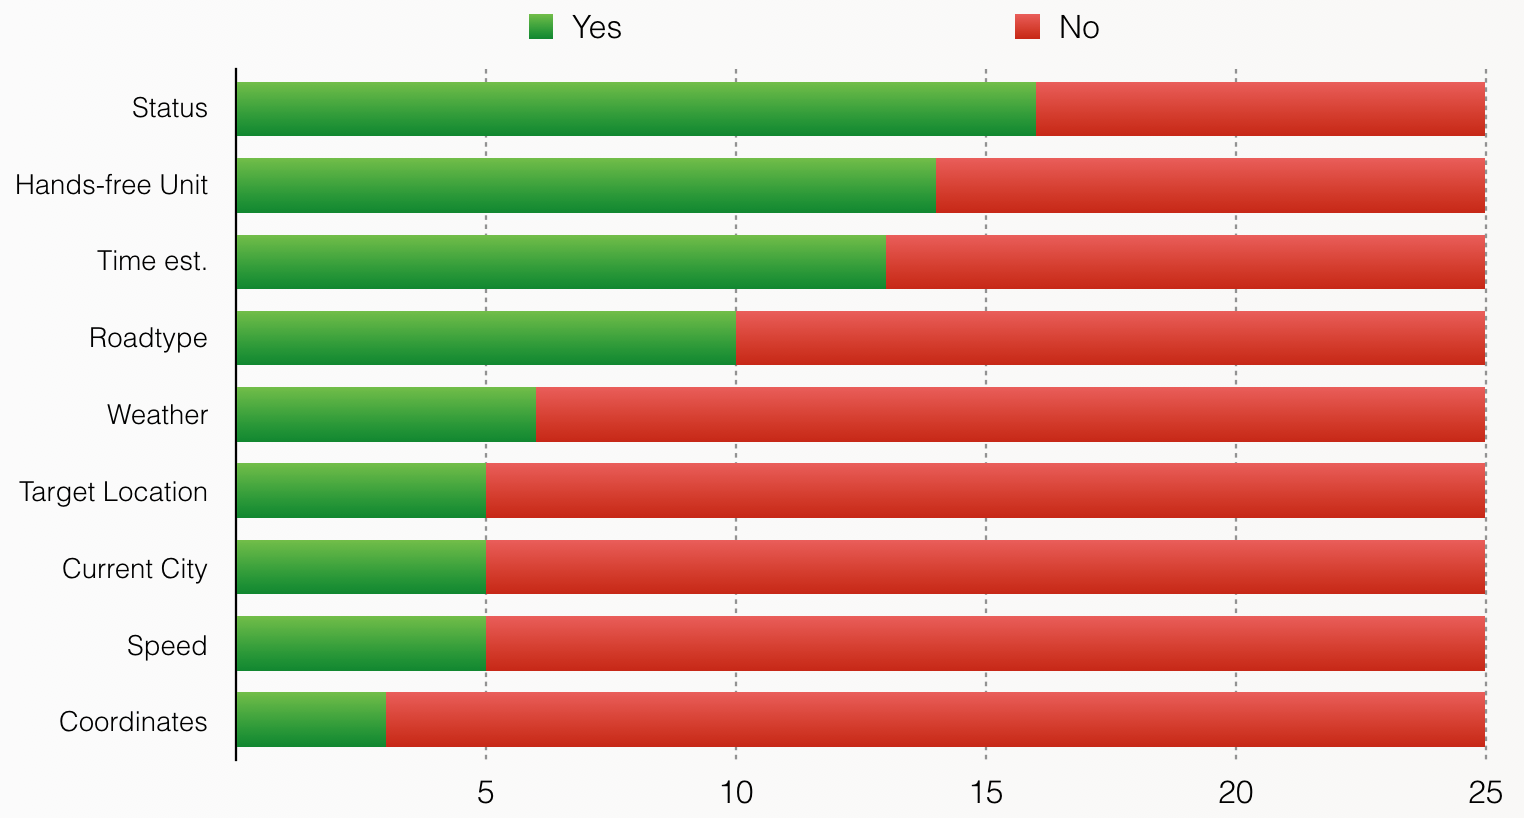
\includegraphics[width=0.9\columnwidth]{figures/WhatAreYouWillingToShare}
  \caption{User Study: What information are you willing to share}~\label{fig:WhatAreYouWillingToShare}
\end{figure}

In figure \ref{fig:WhatAreYouWillingToShare}


\section{Conclusion and Future Work}

TODO: put text here

\section{Acknowledgments}

Sample text: We thank all the volunteers, and all publications support
and staff, who wrote and provided helpful comments on previous
versions of this document. Authors 1, 2, and 3 gratefully acknowledge
the grant from NSF (\#1234--2012--ABC). \textit{This whole paragraph is
  just an example.}

 Balancing columns in a ref list is a bit of a pain because you
 either use a hack like flushend or balance, or manually insert
 a column break.  http://www.tex.ac.uk/cgi-bin/texfaq2html?label=balance
 multicols doesn't work because we're already in two-column mode,
 and flushend isn't awesome, so I choose balance.  See this
 for more info: http://cs.brown.edu/system/software/latex/doc/balance.pdf

 Note that in a perfect world balance wants to be in the first
 column of the last page.

 If balance doesn't work for you, you can remove that and
 hard-code a column break into the bbl file right before you
 submit:

 http://stackoverflow.com/questions/2149854/how-to-manually-equalize-columns-
 in-an-ieee-paper-if-using-bibtex

 Or, just remove \balance and give up on balancing the last page.

\balance{}

\section{References Format}
Your references should be published materials accessible to the
public. Internal technical reports may be cited only if they are
easily accessible and may be obtained by any reader for a nominal
fee. Proprietary information may not be cited. Private communications
should be acknowledged in the main text, not referenced (e.g.,
[Golovchinsky, personal communication]). References must be the same
font size as other body text. References should be in alphabetical
order by last name of first author. Use a numbered list of references
at the end of the article, ordered alphabetically by last name of
first author, and referenced by numbers in brackets. For papers from
conference proceedings, include the title of the paper and the name of
the conference. Do not include the location of the conference or the
exact date; do include the page numbers if available. 

References should be in ACM citation format:
\url{http://www.acm.org/publications/submissions/latex_style}.  This
includes citations to Internet
resources~\cite{CHINOSAUR:venue,cavender:writing,psy:gangnam}
according to ACM format, although it is often appropriate to include
URLs directly in the text, as above. Example reference formatting for
individual journal articles~\cite{ethics}, articles in conference
proceedings~\cite{Klemmer:2002:WSC:503376.503378},
books~\cite{Schwartz:1995:GBF}, theses~\cite{sutherland:sketchpad},
book chapters~\cite{winner:politics}, an entire journal
issue~\cite{kaye:puc},
websites~\cite{acm_categories,cavender:writing},
tweets~\cite{CHINOSAUR:venue}, patents~\cite{heilig:sensorama}, 
games~\cite{supermetroid:snes}, and
online videos~\cite{psy:gangnam} is given here.  See the examples of
citations at the end of this document and in the accompanying
\texttt{BibTeX} document. This formatting is a edited version of the
format automatically generated by the ACM Digital Library
(\url{http://dl.acm.org}) as ``ACM Ref.'' DOI and/or URL links are
optional but encouraged as are full first names. Note that the
Hyperlink style used throughout this document uses blue links;
however, URLs in the references section may optionally appear in
black.

 BALANCE COLUMNS
\balance{}

 REFERENCES FORMAT
 References must be the same font size as other body text.
\bibliographystyle{SIGCHI-Reference-Format}
\bibliography{sample}

\end{document}

 Local Variables:
 mode: latex
 TeX-master: t
 End:
